\chapter{Prove di Performance}
\section{Versione sequenziale e versione concorrente}
Sono state effettuate diverse prove di esecuzione utilizzando anche macchine con hardware diversi. In ogni caso, la versione sequenziale del programma risulta più lenta ed inefficiente della sua versione concorrente.\newline

\noindent Al fine di poter effettuare tali prove, il nostro algoritmo è stato astratto in un metodo invocabile dove, tra i vari argomenti, viene fornito il numero di Worker che vi si vuole dedicare. Se nella versione concorrente si è scelto di dedicare \textbf{N Worker} (con N corrispondente al numero di processori disponibili sulla macchina), nella versione sequenziale semplicemente viene dedicato un solo Worker, ottenendo di fatto un esecuzione sequenziale.

\noindent Ai fini di questo report, le statistiche riportate fanno riferimento ad un'architettura con queste specifiche:
\begin{itemize}
    \item Intel(R) Core(TM) i5-2520M CPU @ 2.50GHz, 2 Core, 4 Thread, 3 MB Intel® Smart Cache
    \item 8 GB Ram
\end{itemize}

\noindent Questi sono i risultati per la versione sequenziale dell'algoritmo
\begin{figure}[H]
	\begin{center}
		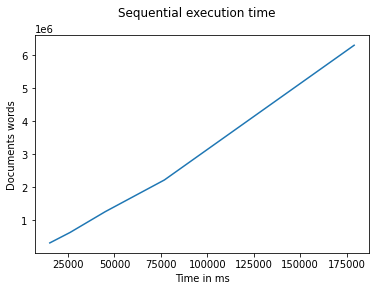
\includegraphics[width=0.55\linewidth]{img/sequential-graph.png}
		\label{fig:seq}
		\caption{Grafico delle prestazioni, algoritmo sequenziale}
	\end{center}
\end{figure}

\noindent Mentre questi sono i risultati della versione parallelizzata:
\begin{figure}[H]
	\begin{center}
		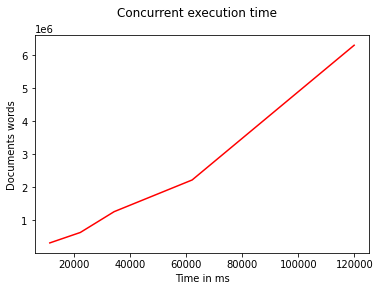
\includegraphics[width=0.55\linewidth]{img/concurrent-graph.png}
		\label{fig:conc}
		\caption{Grafico delle prestazioni, algoritmo concorrente}
	\end{center}
\end{figure}

\noindent Per un migliore confronto delle prestazioni ecco i due risultati sovrapposti:

\begin{figure}[H]
	\begin{center}
		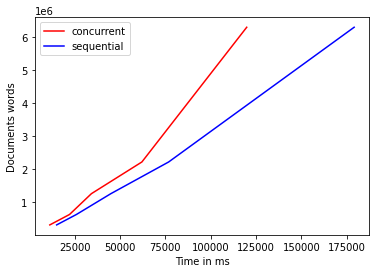
\includegraphics[width=0.55\linewidth]{img/concurrent-vs-sequential-graph.png}
		\label{fig:seqconc}
		\caption{Grafici delle prestazioni a confronto}
	\end{center}
\end{figure}

\noindent Come si può evincere dai grafici, questa versione non migliora di molto le performance con un numero basso di documenti (in particolar modo quando il numero di documenti da analizzare è minore rispetto al numero di processori disponibili sulla macchina), ma ottiene risultati molto soddisfacenti quando i documenti da analizzare sono invece molteplici.\newline

\noindent Lo \textbf{speedup} è un indice che permette di quantificare il miglioramento delle prestazioni di un sistema, mettendo in relazione il tempo di esecuzione nel caso sequenziale e nel caso concorrente (con l'impiego di N thread).\newline
La formula per calcolare lo speedup è la seguente:
$$ S = \frac{T_1}{T_N} \; \xrightarrow{in\;our\;scenario} S = \frac{T_1}{T_4}$$


$$ S = \frac{179084\;ms}{119889\;ms} = 1,4938 \approx$$
\section{Performance di versioni alternative}
Durante lo sviluppo di questo applicativo, sono emerse alcune questioni che hanno fatto mutare l'architettura in corso d'opera.\newline

\noindent Il primo fattore da considerare è il caricamento in memoria centrale dei documenti. Tale operazione risulta limitatamente parallelizzabile in quanto un singolo documento dev'essere caricato interamente e tale operazione non è decomponibile in porzioni più piccole. Esso risulta dunque un grande collo di bottiglia per le performance. L'unica parallelizzazione possibile dunque, consiste nel caricare in memoria più documenti contemporaneamente tramite thread diversi.\newline

\noindent La seconda questione invece ha natura più algoritmica. Una volta caricato il documento in memoria e suddiviso in pagine, sarebbe possibile eseguire il conteggio delle parole in modo parallelo. A tale scopo avevamo sviluppato due soluzioni che facevano esattamente ciò, ma con risultati considerevolmente peggiori in quanto a performance.

\subsection{Versione alternativa 1: Divisione in più Task}
Nella prima implementazione da noi sperimentata, abbiamo adottato l'approccio che più ci è sembrato naturale; il ComputeFileTask era dunque suddiviso in 2 sotto-task:
\begin{itemize}
    \item \textbf{ReadFileTask}\newline
    Responsabile del caricamento in memoria centrale del documento e della sua suddivisione in "Pagine". Per ogni Pagina veniva dunque creato ed aggiunto alla Bag of Tasks un PageTask.
    \item \textbf{PageTask}\newline
    Si occupava di analizzare il contenuto di una Pagina, contando le istanze delle parole. Una volta analizzata tutta la Pagina, il risultato veniva salvato nella struttura centrale.
\end{itemize}
Questa soluzione divide sicuramente in maniera più equa il lavoro nel caso di un ridotto numero di documenti. \newline

\noindent Prendiamo, ad esempio, un documento PDF di 10 pagine. Con questa soluzione un singolo thread si occuperà del caricamento e della suddivisione in pagine, ma molteplici thread eseguiranno il conto delle istanze delle parole nelle 10 pagine.\newline

\noindent Durante l' analisi delle prestazioni, però, ci siamo rapidamente resi conto che, con grandi quantità di documenti, una minor suddivisione in pagine migliorava notevolmente le performance; riprendendo l'esempio di prima sarebbe stato possibile, ad esempio, suddividere il documento in 5 pagine, ottenendo di conseguenza 5 PageTask piuttosto che 10.\newline

\noindent Ulteriori test ci hanno portato a concludere che, per grandi quantità di documenti, si ottenevano performance migliori unificando i due Task.\newline

\noindent Il problema della prima versione alternativa dunque è da individuarsi nell'elevato numero di accessi a porzioni di codice per cui è richiesta la sincronizzazione tra processi:
\begin{itemize}
    \item Deposito dei nuovi Task nella Bag of Tasks (uno per ogni nuovo PageTask)
    \item Prelievo di un numero molto maggiore di Task dalla Bag of Task (il numero di documenti sommato al numero totale di pagine nei documenti, supponendo una suddivisione massima delle pagine)
    \item Aggiornamento della struttura centrale contenente il risultato (uno per ogni PageTask che abbia concluso l'elaborazione)
\end{itemize}

\noindent Era inoltre richiesta un'ulteriore struttura di sincronizzazione necessaria a stabilire una condizione di terminazione: il completamento di tutti i ReadFileTask.
Risultava possibile, infatti, che in alcuni momenti la Bag of Task fosse vuota, ma alcuni Worker stessero ancora elaborando qualche ReadFileTask (dai quali sarebbero stati prodotti nuovi PageTask). Attraverso questa struttura di sincronizzazione dunque era possibile stabilire se mettere in attesa un Worker che richiedesse un Task dalla Bag of Tasks vuota o se permettergli di terminare la sua esecuzione richiedesse un nuovo Task da eseguire.\newline

\noindent Tale struttura dunque richiedeva un ulteriore sforzo di sincronizzazione che deteriorava le performance. Nella versione finale questo meccanismo non risulta più necessario in quanto una Bag of Tasks vuota coincide necessariamente con la fine dell'esecuzione (dato che esistono solo ComputeDocumentTask).

\subsection{Versione alternativa 2: Ulteriore layer di master-workers}
Riprendendo la soluzione precedente, un altro tentativo di parallelizzazione è stato svolto (traendo spunto dalla teoria) espandendo i master-workers, rendendo i worker a loro volta master.\newline

\noindent Un Worker, una volta preso in carico un ReadFileTask, suddivideva il documento in un numero ragionevole di pagine (ad esempio N, con N uguale al numero di processori disponibili); per ogni pagina creata, veniva dunque istanziato (attraverso fork-join) un nuovo Worker che avrebbe eseguito il PageTask.\newline

\noindent Il motivo per cui, in questo particolare progetto, le performance peggioravano, è da ricercarsi nelle tempistiche di elaborazione contrapposte a quelle della creazione di nuovi thread.\newline

\noindent Il conteggio delle parole, difatti, richiede un tempo molto basso (la maggior parte del tempo di esecuzione è occupata dal caricamento in memoria dei documenti) che non giustifica i ritardi dovuti alla creazione e sincronizzazione di nuovi thread.

\subsection{In conclusione sulle performance}
Questo progetto ci ha permesso di toccare con mano la realtà della programmazione concorrente, scontrandoci con tematiche molto concrete.\newline

\noindent La granularità con la quale suddividere la computazione non è universale, ma è fortemente influenzata dalle caratteristiche dell'applicativo: in alcuni casi una maggiore suddivisione del lavoro potrà essere un approccio vincente, ma in altri la necessità di una maggiore sincronia tra processi potrebbe portare ad un decremento nelle performance.
